\subsection{The Observer}
The previous section assumed that the state variables can be modeled, which is not necessaryily the case. To make
it interesting I am going to assume that the system's velocities can be measured(ie only relative encoders are
available for the system).

This is going to create a c matrix of:
\begin{equation}
\begin{bmatrix}
1 & 0 & 0 & 0 & 0 & 0\\
0 & 1 & 0 & 0 & 0 & 0\\
0 & 0 & 1 & 0 & 0 & 0
\end{bmatrix}\end{equation}


The desired eigenvalues are 3 times the controller eigenvalues
in order to allow the observer to converge faster than the controller, this resulted in:\begin{enumerate}
  \item $(-9+9j)$
  \item $(-9-9j)$
  \item $(-10.5+10.5j)$
  \item $(-10.5-10.5j)$
  \item $(-12+12j)$
  \item $(-12-12j)$
\end{enumerate}
The first goal will be to reduce the multi-output model to a single
output model
the desired eigenvalues for the observer are: 
\begin{equation}
\lambda = (-9+9j), (-9-9j), (-10.5+10.5j), (-10.5-10.5j), (-12+12j), (-12-12j)
\end{equation}
Desired Characteristic equation
\begin{equation}
\Delta_d(\lambda) = \lambda^{6} + 63.0 \lambda^{5} + 1984.5 \lambda^{4} + 36855.0 \lambda^{3} + 431649.0 \lambda^{2} + 2980152.0 \lambda + 10287648.0
\end{equation}
Desired Characteristic equation
\begin{equation}
\bar \alpha = \left[\begin{matrix}10287648.0\\2980152.0\\431649.0\\36855.0\\1984.5\\63.0\end{matrix}\right]
\end{equation}
Desired Characteristic equation
\begin{equation}
\Delta_d(\lambda) = \operatorname{PurePoly}{\left( 1.0 \lambda^{6} + 0.2750244140625 \lambda^{5} - 14.6950073242188 \lambda^{4} - 1.71600341796875 \lambda^{3} - 48.1669921875 \lambda^{2}, \lambda, domain=\mathbb{R} \right)}
\end{equation}
Desired Characteristic equation
\begin{equation}
\alpha = \left[\begin{matrix}0\\0\\-48.167\\-1.716\\-14.695\\0.275\end{matrix}\right]
\end{equation}
$\bar l$
\begin{equation}
  \bar l = \bar \alpha - \alpha = 
\end{equation}
\begin{equation}
  \bar l = \left[\begin{matrix}10287648.0\\2980152.0\\431649.0\\36855.0\\1984.5\\63.0\end{matrix}\right] - \\\left[\begin{matrix}0\\0\\-48.167\\-1.716\\-14.695\\0.275\end{matrix}\right] = 
\end{equation}
\begin{equation}
  \bar l = \left[\begin{matrix}10287648.0\\2980152.0\\431697.167\\36856.716\\1999.195\\62.725\end{matrix}\right]
\end{equation}
Calculate P
\begin{equation}
 Q = P.T = 
  \begin{bmatrix}
    (A.T)^5C.T & (A.T)^4C.T & (A.T)^3C.T & (A.T)^2C.T & (A.T)C.T & C.T\\
  \end{bmatrix}
  \begin{bmatrix}
    1 & 0 & 0 & 0 & 0 & 0\\
    \alpha_1 & 1 & 0 & 0 & 0 & 0\\
    \alpha_2 & \alpha_1 & 1 & 0 & 0 & 0\\
    \alpha_3 & \alpha_2 & \alpha_1 & 1 & 0 & 0\\
    \alpha_4 & \alpha_3 & \alpha_2 & \alpha_1 & 1 & 0\\
    \alpha_5 & \alpha_4 & \alpha_3 & \alpha_2 & \alpha_1 & 1\\
  \end{bmatrix}
\end{equation}\begin{equation}
  Q = \left[\begin{matrix}0 & 0 & 0 & 0 & 0 & 1.84\\119.414 & -354.53 & 3.34 & -15.827 & 0 & 1.163\\-33.035 & 77.876 & -1.63 & 12.344 & 0 & 1.518\\78.499 & -3.658 & 12.358 & -0.094 & 1.518 & 0\\-355.139 & 5.147 & -15.844 & 0.081 & 1.163 & 0\\0.337 & -0.794 & 0.017 & -0.126 & 1.84 & 0\end{matrix}\right]\left[\begin{matrix}1 & 0 & 0 & 0 & 0 & 0\\0 & 1 & 0 & 0 & 0 & 0\\0 & 0 & 1 & 0 & 0 & 0\\-48.167 & 0 & 0 & 1 & 0 & 0\\-1.716 & -48.167 & 0 & 0 & 1 & 0\\-14.695 & -1.716 & -48.167 & 0 & 0 & 1\end{matrix}\right]
\end{equation}
\begin{equation}
  Q = \left[\begin{matrix}-27.038 & -3.158 & -88.625 & 0 & 0 & 1.84\\864.638 & -356.527 & -52.689 & -15.827 & 0 & 1.163\\-649.936 & 75.27 & -74.757 & 12.344 & 0 & 1.518\\80.404 & -76.785 & 12.358 & -0.094 & 1.518 & 0\\-361.021 & -50.882 & -15.844 & 0.081 & 1.163 & 0\\3.24 & -89.419 & 0.017 & -0.126 & 1.84 & 0\end{matrix}\right]
\end{equation}
\begin{equation}
  P = Q.T = \left[\begin{matrix}-27.038 & 864.638 & -649.936 & 80.404 & -361.021 & 3.24\\-3.158 & -356.527 & 75.27 & -76.785 & -50.882 & -89.419\\-88.625 & -52.689 & -74.757 & 12.358 & -15.844 & 0.017\\0 & -15.827 & 12.344 & -0.094 & 0.081 & -0.126\\0 & 0 & 0 & 1.518 & 1.163 & 1.84\\1.84 & 1.163 & 1.518 & 0 & 0 & 0\end{matrix}\right]
\end{equation}
\begin{equation}
  l = P^{-1} \bar l  = \left[\begin{matrix}16931.654\\-11720.663\\-11498.595\\-14541.918\\-40028.382\\38391.429\end{matrix}\right]
\end{equation}
\begin{equation}
  L = lv  = \left[\begin{matrix}31153.499 & 19695.321 & 25705.401\\-21565.505 & -13633.767 & -17794.148\\-21156.909 & -13375.452 & -17457.007\\-26756.489 & -16915.52 & -22077.336\\-73650.464 & -46562.011 & -60770.532\\70638.542 & 44657.866 & 58285.332\end{matrix}\right]
\end{equation}
The final values of this ended up as follows: 
\begin{equation}
\vert A-LC \vert = 
\left[\begin{matrix}-31153.499 & -19695.321 & -25705.401 & 0 & 0 & 1.0\\21565.505 & 13633.767 & 17794.148 & 0 & 1.0 & 0\\21156.909 & 13375.452 & 17457.007 & 1.0 & 0 & 0\\26756.489 & 16905.71 & 22077.336 & -0.1 & 0.05 & 0\\73650.464 & 46576.726 & 60765.627 & 0.05 & -0.075 & 0.05\\-70638.542 & -44667.676 & -58275.522 & 0 & 0.05 & -0.1\end{matrix}\right]\end{equation}
\begin{enumerate}
  \item $-15.833 - 15.011 i$
  \item $-7.404 - 13.269 i$
  \item $-5.044$
  \item $-11.483$
  \item $-7.404 + 13.269 i$
  \item $-15.833 + 15.011 i$
\end{enumerate}
Ya that isn't the best, but considering this is a 6 variablesystem, im calling it close enough
\begin{figure}[H]
  \begin{center}
    \makebox[\textwidth]{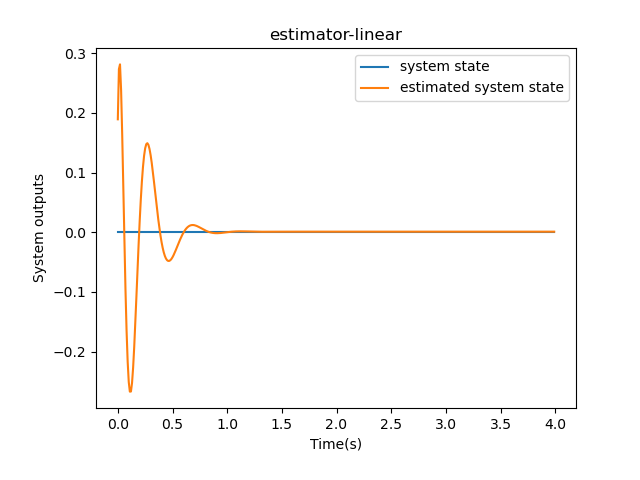
\includegraphics[max width=\textwidth]{../resources/estimator-linear.png}}
  \end{center}
  \caption{Estimator in Linear performance}
  \label{fig:estimator-linear}
\end{figure}


For the next two plots, I was not able to get the observer to converge fast enough, with little overshoot
in order to cause the system to be stable. I know parrallel axis theorem is a thing, and I cannot explain it,
so for the next two plots, the feedback is given the true state rather than the estimated state.
\begin{figure}[H]
  \begin{center}
    \makebox[\textwidth]{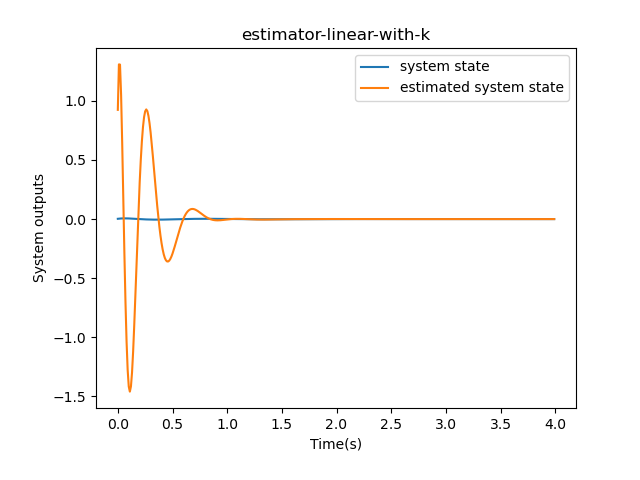
\includegraphics[max width=\textwidth]{../resources/estimator-linear-with-k.png}}
  \end{center}
  \caption{Estimator in Linear performance}
  \label{fig:estimator-linear-with-k}
\end{figure}

\begin{figure}[H]
  \begin{center}
    \makebox[\textwidth]{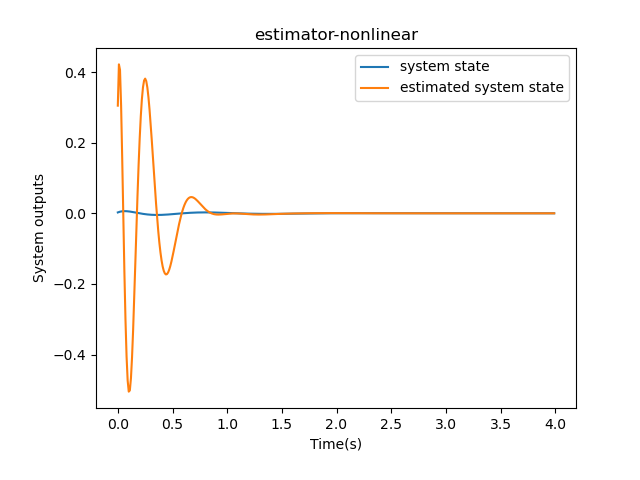
\includegraphics[max width=\textwidth]{../resources/estimator-nonlinear.png}}
  \end{center}
  \caption{Estimator in NonLinear performance}
  \label{fig:estimator-nonlinear}
\end{figure}
